\chapter{Design and development} \label{chap:designanddev}
Based on the requirements defined in the previous section, this chapter covers the design and the subsequent development of the solution. While the first section presents the preparatory steps leading to the final design of the artifact, the latter section presents the choices that are made regarding technology, development environment and implementation to transform the artifact from a simple design to a working solution.

\section{Designing the artifact} \label{sec:ArtifactDesign}
The first step of the design process consists of specifying the flow of the information. As discussed in \ref{sec:InformationPresentation}, there is no rigid, predefined way of introducing the different concepts to the audience. Instead, it is upon the author to lead the user through the explanation. The chosen approach divides the artifact into two parts: the guided tour and the overview. This division lets the user decide whether to follow the guided tour which presents a high-level introduction to the different topics (and then leads to the overview) or whether to jump straight to the overview which presents these topics, too, but in a more detailed and interactive manner. The following paragraphs now deal with the guided tour before the structure of the overview is presented.

\paragraph{Guided tour} Taking into account the requirements from \ref{sec:ReqSpec}, figure \ref{fig:DesignConcept} presents the flow of information. %It is for this reason that the following graphic (figure \ref{fig:DesignConcept}) is developed which presents the flow of information.
While the number of boxes behind a topic indicates how much text there will be in the final design, any more detailed information is omitted and is presented in an ensuing step. 

\begin{figure}
 \centering
 \includesvg[width=0.8\linewidth]{graphics/DesignConceptSteps.svg}
 \caption{Flow of the presented information during the guided tour}
    \label{fig:DesignConcept}
\end{figure}

Keeping in mind that the target audience has only little to no knowledge about blockchain technology, the information is presented within a narrative context. With the help of two fictional actors, Anna and Bob, the audience is presented with a summary of the financial aspect of cryptoeconomics. This includes a brief description of the role of money, the role of banks, the process of transferring money between parties and finally how new technologies have affected the way money is accessed and distributed. After explaining how traditional system transfer money, the concept of distributed systems is introduced in the form of multiple bank symbols representing a decentralized peer to peer transaction system. Nodes (participants in that network) and their different types are presented, and it is shown how Anna and Bob would interact with that system instead of a centralized system. An important information is also the way the distributed system reaches a shared state as compared to a centralized system. By providing a concrete comparison between these two systems (centralized and distributed), the user should be able to recognize the difference more easily. After presenting the nodes, it must be made clear why the system should behave a certain way. As this is based on game-theoretic concepts, the story introduces them subsequently: By continuing the storyline of Anna and Bob (what happens if Anna's node is malicious and wants to hurt the network?), it is shown that a node is incentivized to act in favour of the overall system as that is in its interest. Once these three concepts, constituting the three pillars of cryptoeconomics, have been introduced, the concept of public and private key infrastructure is presented by showing how Anna and Bob both use their key pairs to create transactions in the network. The concept of transactions then guides the user to one of the major technical characteristics of blockchain: the blocks and the cryptographic hash functions that link those blocks to form an immutable chain of transactions. As indicated in figure \ref{fig:DesignConcept}, this part of the explanation is most likely to need the most text. This topic is then followed by the presentation of consensus mechanisms which are used to attain the same state for every node in the network. Note that this part of the explanation appends to the topic of distributed systems (one shared state) in a way that the presented consensus mechanisms are specific to blockchain, whereas other distributed systems use a different mechanism to reach their shared state. Finally, the guided tour leads to a presentation of different use cases that blockchain enables. The user sees a list of various use cases with which they may interact to learn more. These use cases should be as easy to understand as possible to facilitate meaningful learning and to support the user in addressing possible use cases (specific to their position) more precisely.

Albeit the segmenting principle states that different concepts should be presented independently of each other, uncoupling these closely intertwined concepts from each other would prove harmful to the learning experience because the user would miss the context in which the specific concept is situated. Therefore, since repetitions cannot be avoided entirely, this thesist intends to limit them in such a way that the explanation is not repetitive but presents a well rounded and easy to understand explanation of this complex technology.

\paragraph{Overview} At the end of the guided tour, the user is presented with the overview, presented in figure \ref{fig:OverviewPic}, which allows more in-depth insights into specific concepts.
In this overview, the audience is free to decide about which of the concepts they want to learn more. They are also given the opportunity to test out the concepts, such as playing with hashed values or changing the content of a block within the existing blockchain (see requirement 28a-c).

\begin{figure}
    \centering
    \includesvg[width=0.8\linewidth]{graphics/Blockchain_Overview.svg}
    \caption{Preliminary sketch of the overview section}
    \label{fig:OverviewPic}
\end{figure}

After the flow of information is defined, a rough sketch of the different screens the user is led through is drawn on paper. The rough draft serves as the basis for the development, and it is used to ensure that the requirements are included in the artifact.\footnote{As the sketches cannot portray which technology is used and what graphical design decisions are made (requirements 12 - 14 and 29 to 31), the actual requirements specification should be regarded during the development process, too.} The development of the artifact is described in the following section.

\section{Developing the artifact}

As a first task, before the actual task of implementing the artifact may begin, a technology needs to be identified that meets the requirements 29 to 31. The solution should be location independent, process user interactions and should be easily adapted by other developers to be applied in different situations.\footnote{This means that the different use cases presented in the overview may be changed to accommodate a specific industry.} A possible solution is that of a web application due to its wide spread use, easy portability, easy deployment and the fact that changes may be easily implemented as the programming/scripting languages HTML, CSS and JavaScript are a common skill set among web developers. When following this approach, (regardless of whether the files are on a local machine or the web site is hosted online) the artifact is accessed via the browser allowing a quick set-up. This approach additionally allows the artifact's presentation from a remote location, if needed.

A first prototype of the artifact is developed within the web-based editor WebFlow. The editor allows the visual manipulation of code and changes to the CSS are reflected in real-time in the web preview of the editor). With this feature, the general style of the artifact's elements is quickly defined. The first prototype consists of a pop-up window which includes paragraphs of text and a button, as illustrated in figure \ref{fig:proto1}. WebFlow also allows to create simple interactions, so when the user hovers over the button or clicks it, the button gives visual feedback (changes in shadow style and upwards movement).

\begin{figure}
    \centering
    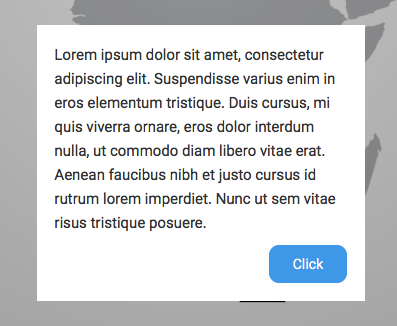
\includegraphics[width=0.4\textwidth]{latex-vorlage_v1.5/graphics/Prototype1.png}
    \caption{Prototypical pop-up window, styled in WebFlow}
    \label{fig:proto1}
\end{figure}

During the prototyping in WebFlow and the ensuing development of the artifact in the text editor Atom, the design considerations in the form of the paper sketches and the requirements specification are continuously taken into consideration so that the final artifact presents a complete instantiation of the defined solution space.

The landing page (index.html) of the web page consists of two simple buttons which redirect either to the guided tour (guided-tour.html) or the overview (overview.html) (as illustrated in figure \ref{fig:ButtonStyle}, corresponding to requirement 19). In order to ensure consistent style, all pages access a shared CSS file and classes are defined to which the elements are assigned (such as the buttons of \texttt{class = "ButtonsMain"}). 

\begin{figure}
    \centering
    \includesvg[width=\textwidth]{graphics/protoAll.svg}
    \caption{Buttons, styled by \texttt{.ButtonsMain}, on the landing page redirect to either the tutorial or the overview}
    \label{fig:ButtonStyle}
\end{figure}

\paragraph{The guided tour} Once the user has clicked on the button \textit{Let's start the tour}, they view a short intro to the guided tour, stating its purpose and informing the user that the tour continues by clicking on the button on the bottom right of the ensuing pop-up windows (requirement 21). The purpose of this short introduction, written in a thoughtful and friendly manner (corresponding to requirement 25), is to support the user's curiosity, making them more interested in and receptive to the following explanations. Corresponding to the requirements 12-15 and 20, an explanatory paragraph introduces the user to a concept supported by a simple animation visualizing this information. These animations are described in more detail in the following paragraphs while the order of the different concepts corresponds to the information flow of figure \ref{fig:DesignConcept}. The exact wording of these explanations is also not explained in further detail but may generally be described as a high-level summary of the technology, similar to chapter \ref{chap:Blockchain}, but presented in more layman terms.

The tutorial begins with the presentation of the two actors Anna and Bob who accompany the user throughout the tutorial. Figure \ref{fig:Animationline} illustrates the animations in the first part of the tutorial which deals with the financial aspect of cryptoeconomics (requirement 1) and shows how money may be transferred between parties. The dashed arrows and lightly transparent symbols are added to the screen clippings for additional clarity. Firstly, the two actors are introduced (a), then Anna sends Bob money in the form of cash which he receives directly (\ref{fig:Animationline}b). In \ref{fig:Animationline}c, Anna has deposited her capital with a bank which she then orders to transfer money from her account to Bob's. As indicated in the figure, the bank now serves as an intermediary, keeping a small share of the transaction for its service. After this, the user is introduced to the concept of distributed systems (requirement 2), as Anna transfers money to Bob where various nodes in the network process the transaction. It is made clear to the user that all nodes must have the same view of the system to ensure the validity of all transactions. The tutorial continues by explaining how the participating nodes are motivated to participate in favor of the network and how Anna publishes a transaction (requirement 7) by signing it with her private key.

\begin{figure}
    \centering
      \includesvg[width=\textwidth]{graphics/Animations2.svg} 
    \caption{Animations about cryptoeconomics: a) Anna and Bob; b) Anna gives money to Bob directly; c) Anna transfers money to Bob via a bank; d) Anna transfers money to Bob via a distributed system}
    %\caption{Summary of animations inside the guided tour}
    \label{fig:Animationline}
\end{figure}


\begin{figure}
    \centering
      \includesvg[width=\textwidth]{graphics/Animations3Block.svg} 
    \caption{Animating the inclusion of transactions in a block}
    \label{fig:AnimationBlock}
\end{figure}

The tutorial then proceeds with an illustration of how transactions are added to a block, what other data these blocks contain and how they are linked to each other (requirement 3). Figure \ref{fig:AnimationBlock} shows how the transactions are added one after the other inside a container indicating the sender, recipient and amount. Once the container is filled, a pop-up window lists and explains the other data points of a block (time stamp, block number, current and previous block hashes) before a block containig these data points appears and encloses the container with the transactions. When clicked on the button beneath the block, a text box opens in its place leading to the topic of consensus mechanisms. For this, the block is minimized and an animation illustrates the block's propagation throughout the network and its addition to the each node's local version of the blockchain.

Thereafter, the user is led to the final part of the guided tour which presents a summary of different use cases that the blockchain technology enables (requirement 5 and 8). The three different categories of use cases (transactions of value, proof of existence, and automation and machine payments) are situated at the bottom of the page and indicate that they contain more information by slightly changing their style when the user hovers over it (same changes as for the buttons). If clicked upon, the specific element expands to uncover further information and detailed examples of these use cases. Figure \ref{fig:AnimUC} shows the different states: The left element (status:hover) is positioned slightly higher and has a different box shadow (altogether simulating an upwards 3D-movement) than the other elements. While the right element shows no change in style (status:none), the center element is expanded because the user has clicked on it, thus executing a JavaScript function which adds or removes the class \texttt{.expanded} from the element's class list accordingly. The more practical example is presented in two parts: The situation (or problem) and the purpose (argument why blockchain solves this problem). By presenting this example in this simple manner, the user may quickly understand in which situations the blockchain technology might be useful and transfer the information from this concrete example to their field of expertise. Once the user has finished reading through the different use cases, they may go to the overview by clicking on an arrow in the top right stating \textit{Go to the overview} which redirects to \texttt{/overview.html} (requirement 23 and 26). 

\begin{figure}
    \centering
    \includesvg[width=\linewidth]{graphics/AnimationUseCases.svg}
    \caption{The different states of the use case elements}
    \label{fig:AnimUC}
\end{figure}


\paragraph{The overview}
The overview may be considered a natural extension of the guided tour as it offers more detailed information regarding consensus mechanisms, transactions, private and public key cryptography and hash functions. As can be seen in figure \ref{fig:AniOW}, the overview page is of a similar layout as the other pages in the guided tour, but additionally includes a hexagon-shaped element in the center of the distributed system (requirement 18). This element, as well as the icons of Anna and Bob and the up-most block on the blockchain on the right-hand side of the page, provide the entry points for further explanations. The overview, therefore, serves as the center from which all information may be accessed (requirements 17, 24, and 27).\footnote{There is also a link in the top right corner redirecting to the beginning of the guided tour, should the user have skipped it by accident.} To inform the user of these entry points, the elements change their style when the user hovers over them (requirement 14). The change of style is similar to that of the use case elements, described earlier in this chapter. However, the elements also reveal tooltips which intend to motivate the user to click on these elements. For example, the tooltips on the icons of Bob and Anna state \enquote{Learn more about how participants can send transactions} and redirect to the page \texttt{/transactions.html}. This page explains how the user can create their own public and private key pair which they would need to execute a transaction (requirement 10). The second element that offers more information about a shortly presented topic is the hexagon in the center of the page. It leads the user to the page \texttt{/consensus.html} and firstly explains the general role of consensus mechanisms for blockchain technology (requirement 6) and then lists five of the most often implemented consensus mechanisms (proof of work, proof of stake, leased proof of stake, delegated proof of stake, and proof of burn). Since proof of work and proof of stake are the most well-known mechanisms, icons (a pick axe and a vault) depict these mechanisms. All five elements may be expanded individually to reveal more detailed information about the mining techniques if the user wants to know more about these consensus mechanisms. The third element, the newest block in the blockchain, motivates the user to \enquote{learn more about hash functions} as it redirects to the web page \texttt{/hashes.html} (requirement 9). This page explains the nature and purpose of hash functions in more detail. It also explains how a change in a previous block affects its hash value resulting in invalidating all ensuing blocks as they refer to each other by these hashes. This effect is called block mutation effect (requirement 11). However, this site also allows the user to play with these hash functions. They are presented with a text area in which they are instructed to write any arbitrary value (requirement 28). With a click on the button in the center, the input is hashed and presented in the output text area as well as in the element at the bottom which shows the overall history of the session's entered values and corresponding hashes. The history element provides two preset values (\enquote{Hello World} and \enquote{hello world}) which show that even almost identical values result in significantly different hashes. The presented hash values are results of the SHA-256 (Secure Hash Algorithm returning a value of 256 bits) function which is used by the bitcoin implementation. This version is written in JavaScript and takes any ASCII value which it then converts to a SHA-256 hash.\footcite[][]{LuffJavaScriptSHA256demo2014}

\begin{figure}
    \centering
    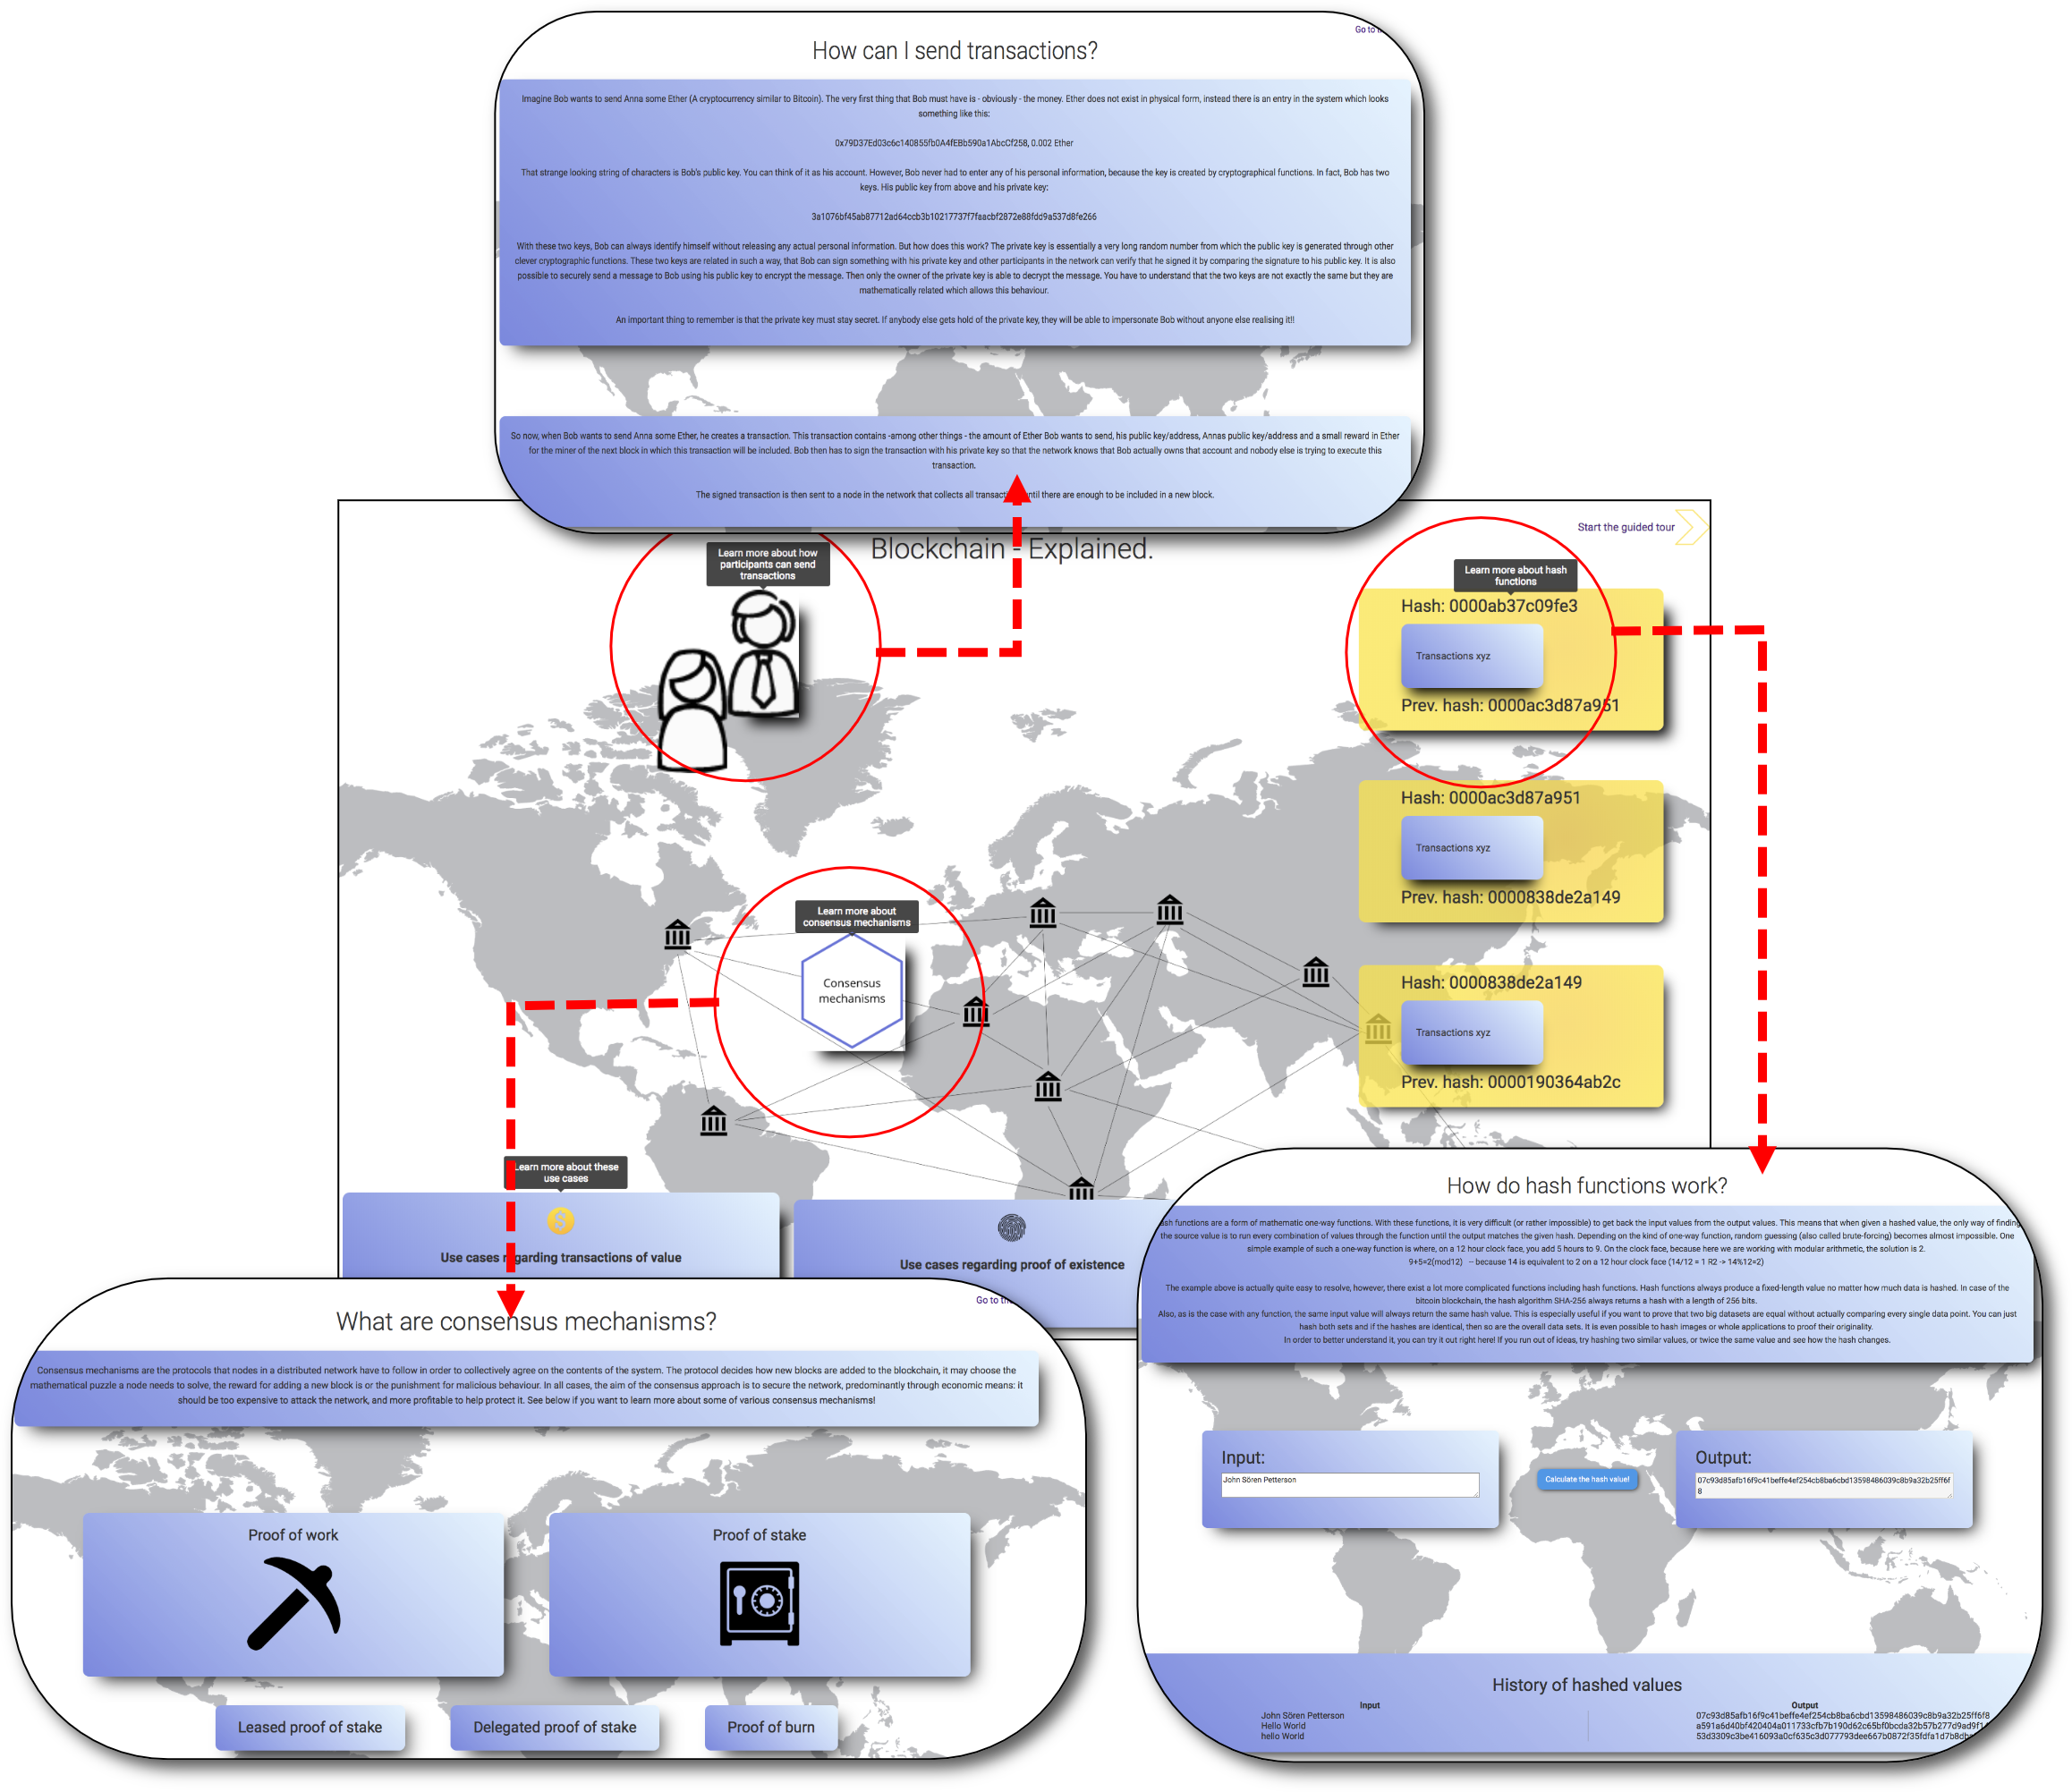
\includegraphics[width=0.7\textwidth]{latex-vorlage_v1.5/graphics/overview.png}
    \caption[The symbols within the overview lead to more information regarding transactions, consensus mechanisms, hash functions and use cases]{The symbols within the overview lead to more information regarding transactions, consensus mechanisms, hash functions and use cases\protect\footnotemark}
    \label{fig:AniOW}
\end{figure}
\footnotetext{A more detailed image can be found in appendix \ref{anhang:OverviewBild}.}

Regarding the requirement of consistent styling (requirement 16), all pages have the same background, consistent font styles, same palette of colour (grey for background and texts, gradient blue for large-area elements and yellow highlights) and a link in the right top corner which either leads to the tutorial (from the overview page) or to the overview (from all other pages). In addition, similar elements (e.g., the buttons or the blue containers) are assigned the same classes so that a change in styling affects all elements equally. Hover effects, as well as on-click-expansion and the revealing of hidden information, are also defined in the CSS file.\footnote{A JavaScript function, called by \texttt{onclick="expand('id')"}, handles the logic of assessing whether a class should be added or removed from the element's class list.} 


Unfortunately, due to constraints in time and resources, it has not been possible to implement more interactive elements similar to that of the hash function (see requirements 28b and c), although the thesis suggests that especially these opportunities to interact with the information allow for meaningful learning to occur. However, the evaluation, described in the following chapter, shall assess how helpful this feature is to the learning experience. If positive, the disregarded features might be included in the next iteration of the artifact. 